\documentclass[tikz]{standalone}

\usepackage[T1]{fontenc}
\usepackage[english]{babel}

\usepackage{graphicx}
\usepackage{standalone}
\usepackage{pgfplots}

\begin{document}
	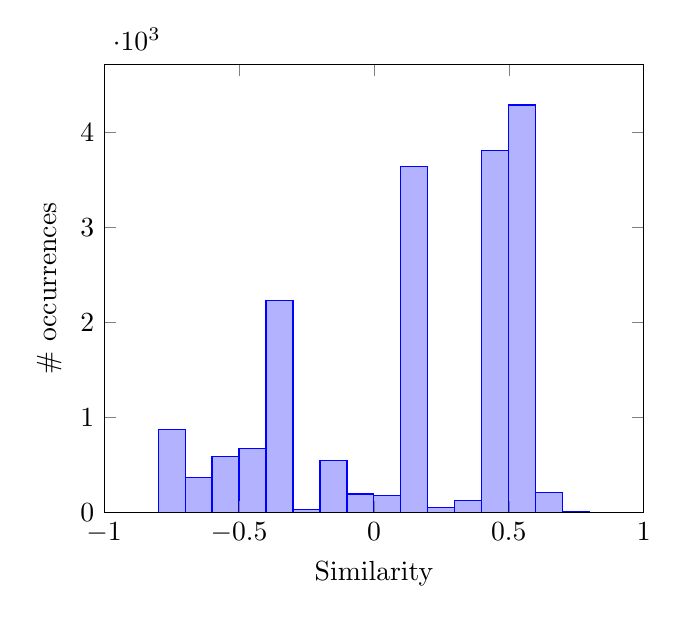
\begin{tikzpicture}
		\begin{axis}[
			ylabel={\# occurrences},
			scaled y ticks={base 10:-3},
			xlabel={Similarity},
			area style,
			axis background/.style={fill=white},
			ymin=0,
			xmin=-1,
			xmax=1
		]
			\addplot+[ybar interval, mark=no] plot coordinates {
				(-1, 0) 
				(-.9, 0)
				(-.8, 876)
				(-.7, 366)
				(-.6, 593)
				(-.5, 675)
				(-.4, 2231)
				(-.3, 33)
				(-.2, 546)
				(-.1, 195)
				(0, 182)
				(.1, 3641)
				(.2, 54)
				(.3, 123)
				(.4, 3815)
				(.5, 4291)
				(.6, 211)
				(.7, 10)
				(.8, 0)
				(.9, 0)
			};
		\end{axis}
	\end{tikzpicture}
\end{document}
